\section{Architecture Integration}

\subsection{Model Support}

\begin{table}[H]
\centering
\small
\begin{tabular}{llllll}
\toprule
\textbf{Model} & \textbf{Attention} & \textbf{Causal?} & \textbf{Nested?} & \textbf{RoPE?} & \textbf{GQA?} \\
\midrule
DistilBERT & \texttt{MultiHeadSelfAttention} & No & No & No & No \\
RoBERTa & \texttt{BertSelfAttention} & No & Yes & No & No \\
GPT-2 & \texttt{GPT2Attention} & Yes & No & No & No \\
Qwen3.5 & \texttt{Qwen3Attention} & Yes & No & Yes & Yes \\
\bottomrule
\end{tabular}
\end{table}

\textbf{Important.} For causal models (GPT-2, Qwen), NEXUS falls back to dense 
attention. The block-sparse path is used only for encoders.

\subsection{Weight Transfer}

\texttt{copy\_weights} extracts via five tiers:

\begin{enumerate}
\item UniversalAdapter
\item GPT-2 Conv1D (chunk)
\item RoBERTa nested (\texttt{self.query})
\item Named projections
\item GQA-aware handling for K/V

\end{enumerate}
\subsection{Nested Encoder Detection}

\begin{lstlisting}
if hasattr(src, "self") and hasattr(getattr(src, "self"), "query"):
    is\_nested = True
elif cls\_name in ("BertSelfAttention", "RobertaSelfAttention") and not has\_out\_proj:
    is\_nested = True
\end{lstlisting}

\subsection{RoPE Support}

Applied to Q, K after projection.

\subsection{GQA Handling}

For K/V with $H_{kv} < H$:

\begin{lstlisting}
if src\_out \textless{} out\_d and out\_d \% src\_out == 0:
    rep = out\_d // src\_out
    target\_w.data.copy\_(w\_oriented.repeat(rep, 1))
\end{lstlisting}

\subsection{RFF Rectification Condition}

The RFF path is active \textbf{only} when:
\begin{itemize}
\item \texttt{layer\_idx \% rectify\_interval == 0}
\item AND (\texttt{pretrained\_attn is None} OR \texttt{enable\_spectraformer=True})

\end{itemize}
Default \texttt{enable\_spectraformer=False} $\to$ RFF inactive.

\subsection{Injection Algorithm}

\textbf{Algorithm 2:} Inject NEXUS
\begin{lstlisting}
Input:  model M, comp\_config
Output: M with attention replaced

1: for   in transformer\_layers(M) do
2:     src $\leftarrow$ get\_attention( )
3:     cfg $\leftarrow$ NEXUSConfig(...)
4:     new $\leftarrow$ NEXUSAttention(model\_config, nexus\_cfg=cfg, pretrained\_attn=src)
5:     replace( , new)
6: end for
\end{lstlisting}

\subsection{Failure Modes}

\begin{table}[H]
\centering
\small
\begin{tabular}{lll}
\toprule
\textbf{Failure} & \textbf{Detection} & \textbf{Response} \\
\midrule
Missing weights & \texttt{missing} non-empty & \textbf{Raise} \\
Near-zero norm & Frobenius & \textbf{Raise} \\
Injection fail & Exception & Log, return None \\
All-negative softpick & \texttt{denom $\approx$ 0} & Uniform (fallback) \\
\bottomrule
\end{tabular}
\end{table}

\subsection{Trainable Parameters}

\begin{itemize}
\item LoRA: all four projections
\item Seer gate: q\_pool, k\_pool
\item RFF proj: when \texttt{is\_rectify=True}

\end{itemize}
\subsection{Registry}

\begin{lstlisting}
@ATTENTION\_REGISTRY.register("nexus", supports\_causal=True, supports\_gqa=True)
class NEXUSAttention(BaseAttention):
    ...
\end{lstlisting}
\begin{lstlisting}

---
\end{lstlisting}

\begin{figure}[H]
\centering
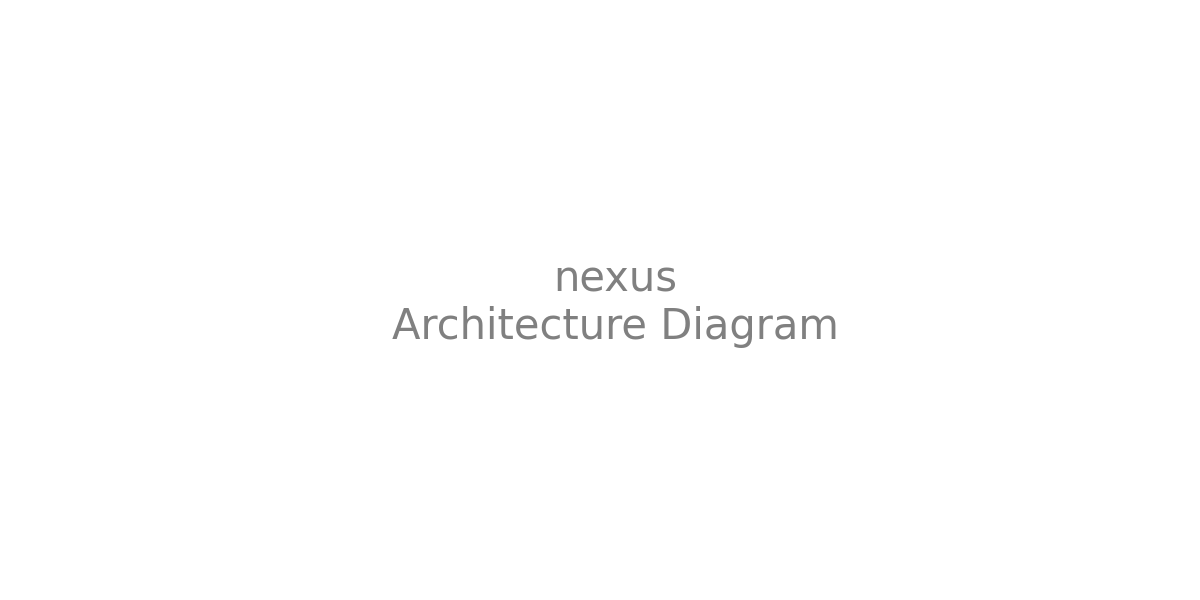
\includegraphics[width=\linewidth]{figures/architecture.png}
\caption{High-level architectural diagram of nexus.}
\label{fig:arch\_nexus}
\end{figure}

